%%%%%%%%%%%%%%%%%%%%%%%%%%%%%%%%%%%%%%%%%%%%%%%%%%%%%%%%%%%%%%%%%%%%
% Einleitung
%%%%%%%%%%%%%%%%%%%%%%%%%%%%%%%%%%%%%%%%%%%%%%%%%%%%%%%%%%%%%%%%%%%%

\chapter{Introduction}
\label{introduction}
- Motivation
%Am Ende der Einleitung folgt ein Text so \"ahnlich wie (Nat\"urlich das folgende alles auf Englisch !!):
%
%Die Arbeit gliedert sich dazu wie folgt: Die Grundlagen von ...
%werden in Kapitel~\ref{introduction} erarbeitet. 
%...
%Eine
%Diskussion und ein kurzer Ausblick im
%Kapitel~\ref{discussion} beschlie{\ss}en diese Arbeit.
%
%Bevor wir uns der Auswertung bzw. Bewertung der gewonnenen Prim\"ardaten zuwenden, wollen wir zun\"achst einige grundlegende Begriffe der deskriptiven Statistik wiederholen.

\section{Background}
\label{background}

	Proteomics is an interdisciplinary research field analyzing the composition, interaction and impacts of the proteome (the entirety of proteins) of single cells or up to a whole organism~\cite{Han2008, Sachsenberg2017}. In this thesis, research was done in a related field, focusing on peptides cross-linked with RNA. The chemical bond between cross-linked molecules has been artificially induced, for example using UV light~\cite{Sachsenberg2017}. Applying this to peptides and RNA could possibly give insight into their \textit{in vivo} interactions, and may also allow conclusions about protein-DNA interaction.\\
	For quantitatively characterizing the proteome of a sample, large scale measuring techniques are needed. Mostly, mass spectrometry (MS) is used, or more specifically, as for the data in this thesis, tandem mass spectrometry (MS/MS) combined with liquid chromatography (LC). In order to analyze the protein sample with MS, its complexity has to be reduced as much as possible, for example using LC~\cite{Sachsenberg2017}. As~\citet{Han2008} explains, the mass spectrometer then produces mass spectra, which have to be analyzed further. It does so by first ionizing the substrate, because it can only detect charged particles. Then, the sample is separated in the mass analyzer by the ratio $\frac{m}{z}$, mass of the particles to their charge. The detector then quantifies the amount of a particle in the sample. The result is a mass spectrum, as shown in figure~\ref{fig:mass_spectrum}.\\
	{
	\renewcommand{\baselinestretch}{0.9} 
	\normalsize
	\begin{figure}
		\centering
		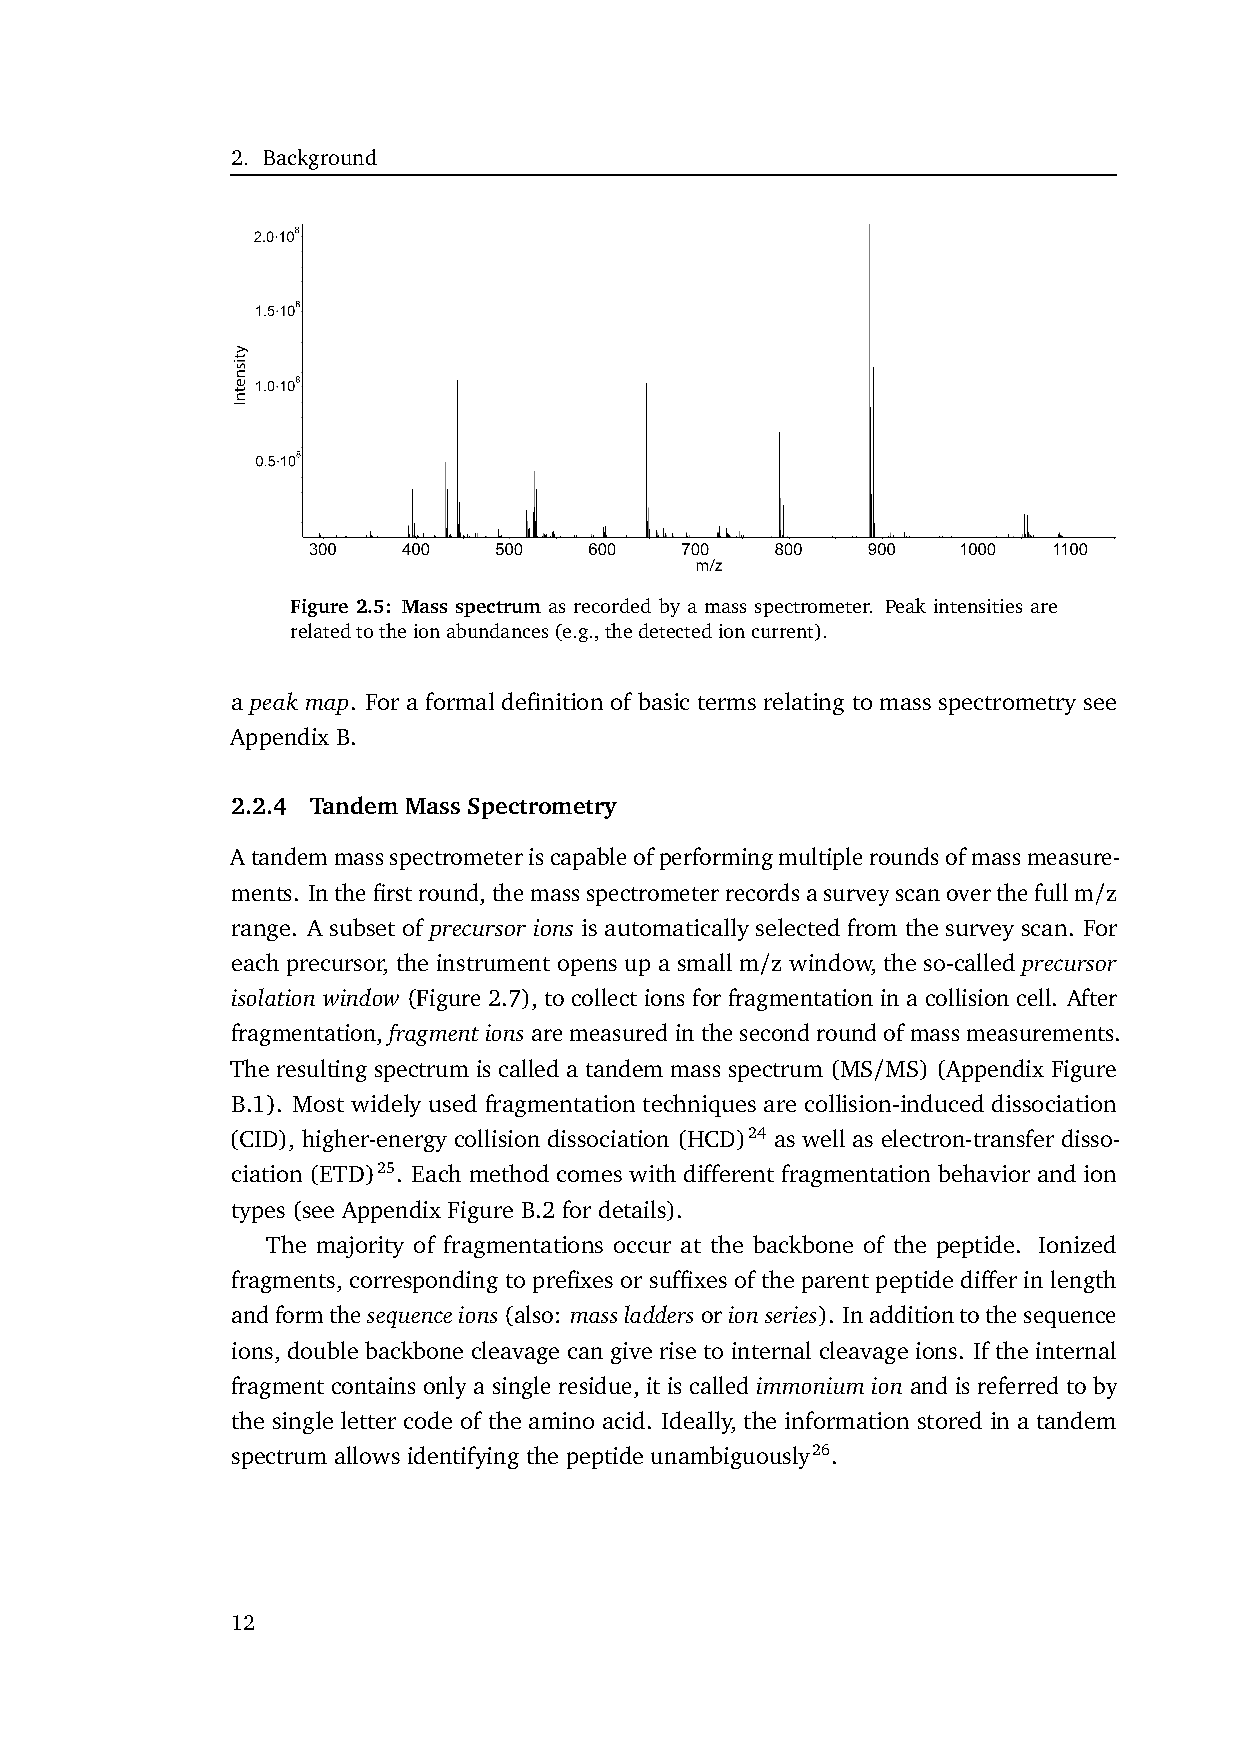
\includegraphics[width = \textwidth, trim=3.9cm 20cm 2.5cm 3cm,clip]{figures/Grafik_Timo.pdf}
		\label{fig:mass_spectrum}
		\caption[Example for a mass spectrum]{Example for a mass spectrum as recorded by a mass spectrometer. The ion intensity correlates with the amount of a molecule in the sample, $\frac{m}{z}$ is the mass-to-charge-ratio. From:~\citet{Sachsenberg2017}}
	\end{figure}
	}
	Because mass alone does not give enough information about a peptide to determine its sequence, tandem mass spectrometry is often used to gather more detailed evidence. In this procedure, particles of similar $\frac{m}{z}$ ratio are selected for fragmentation in a collision cell after the first round of mass measurement~\cite{Sachsenberg2017}. In there, the substance collides with a gas to be broken down into smaller molecules. For proteins, fragmentation happens predominantly in their backbone, producing all possible sub-sequences of the peptide. This produces a spectrum that is almost unique for its protein, which allows for peptide identification using bioinformatics tools~\cite{Angel2012}.\\
	Algorithms like Sequest~\cite{Eng1994} or X!~Tandem~\cite{Craig2004} compare the resulting spectra with theoretical spectra calculated from a list of possible peptides and compute a score based on their similarity. The peptides are generated by obtaining a list of proteins expected in the sample and calculating the peptides resulting from the, for example enzyme-based, degradation of the proteins. The best scoring peptide is then considered a peptide-spectrum-match (PSM). The scores produced by those algorithms often do not distinguish well enough between correct and incorrect matches~\cite{Kll2007}, but they enable FDR estimation using decoy databases and serve as a basis for score re-calibration with the Percolator~algorithm~\cite{Kll2007, Granholm2012}.\\
	Decoy databases are created from the target database, contain usually as  many peptides~\cite{Peng2003, Moore2002} in a reversed or shuffled order with respect to the amino acid sequence~\cite{Aggarwal2016}. They are presented to the scoring algorithm either separately~\cite{Granholm2012} or mixed with the target database~\cite{Peng2003}. It is assumed, that decoy and target peptides have similar features~\cite{Moore2002} and are not easily distinguishable by a scoring algorithm. When the actually fitting peptide for a given spectrum is not in the target database, and thus a wrong one will be chosen, the best scoring peptide will be a decoy approximately half of the time. This allows for an estimation of wrongly assigned targets, since the score distribution is assumed to be the same for decoys and false targets~\cite{Aggarwal2016}.\\
	In practice, one estimates the probability of a PSM being a false target by counting the number of decoy-PSMs with the same or a higher score. It is then assumed, there are as many false targets and thus a false discovery rate (FDR) can be estimated. This leads to the following formula\footnote{In this thesis, the following approximation is used:\\
		$FDR \approx \frac{\text{\# decoy PSMs}}{\text{\# all PSMs}} = \frac{\text{\# decoy PSMs}}{\text{\# decoy PSMs} + \text{\# target PSMs}}$\\
		It is faster to calculate and yields results differing by the FDR, so in the relevant range of FDRs of $0$ to $5\%$ up to $5\%$:\\
		$\frac{\frac{\text{\# decoys}}{\text{\# targets}}}{\frac{\text{\# decoys}}{\text{\# decoys} + \text{\# targets}}} = \frac{\text{\# decoys} + \text{\# targets}}{\text{\# targets}} = 1 + \frac{\text{\# decoys}}{\text{\# targets}} \approx 1 + FDR$}~\cite{Granholm2012}:
	\begin{equation}
	FDR = \frac{\text{\# false target PSMs}}{\text{\# all target PSMs}} \approx  \frac{\text{\# decoy PSMs}}{\text{\# all target PSMs}}
	\end{equation}
	The q-value as a measure for a single PSM rather than a metric for a set of PSMs is then derived from this as the minimum FDR of all PSMs with a lower or equal score~\cite{Granholm2012, Aggarwal2016}. It will be used for estimating the credibility for any one PSM.\\
	As \citet{Kll2007} say, separating correct from incorrect target PSMs with already mentioned algorithms works fine, but there is still room for improvement. This is because often not all information is used and considered jointly. Percolator~\cite{Kll2007, Granholm2012} tries to utilize as much information as possible by using scores from different algorithms, features of the peptide like its length, of the spectrum or the PSM itself. It joins them using a linear SVM and a semi-supervised approach with cross-validation to retain as many PSMs as possible. In every iteration, the top ranking, non-decoy PSMs up to a certain threshold of q-value are chosen as positive training examples, and the decoy PSMs are used as negative training set. The PSMs are then re-ranked using the SVM score, with the intend of getting a better separation of true and false PSMs. If that holds true, the positive training set of the next iteration better is of higher quality and the SVM can be trained even better. The algorithm usually converges within the first 10 iterations~\cite{Kll2007}. To avoid having to split the data into training and testing set and consequently losing possibly correct PSMs but also avoid overfitting, a nested cross-validation approach is being used~\cite{Granholm2012}.


